\documentclass[preview]{standalone}
\usepackage{helvet}
\renewcommand{\familydefault}{\sfdefault}
\usepackage{ulem}

%\usepackage{floatrow}
\usepackage{graphicx}
\graphicspath{{./otherFigures/}}
\usepackage{caption}
\usepackage[label font=bf,labelformat=simple, position = top, justification=RaggedRight,singlelinecheck=false]{subfig}
\newdimen\figrasterwd
\figrasterwd\textwidth
%\floatsetup[figure]{style=plain,subcapbesideposition=top}
\newsubfloat{figure}
\renewcommand{\thesubfigure}{\Alph{subfigure}}


\begin{document}
\begin{figure}
\centering
  \subfloat[][]{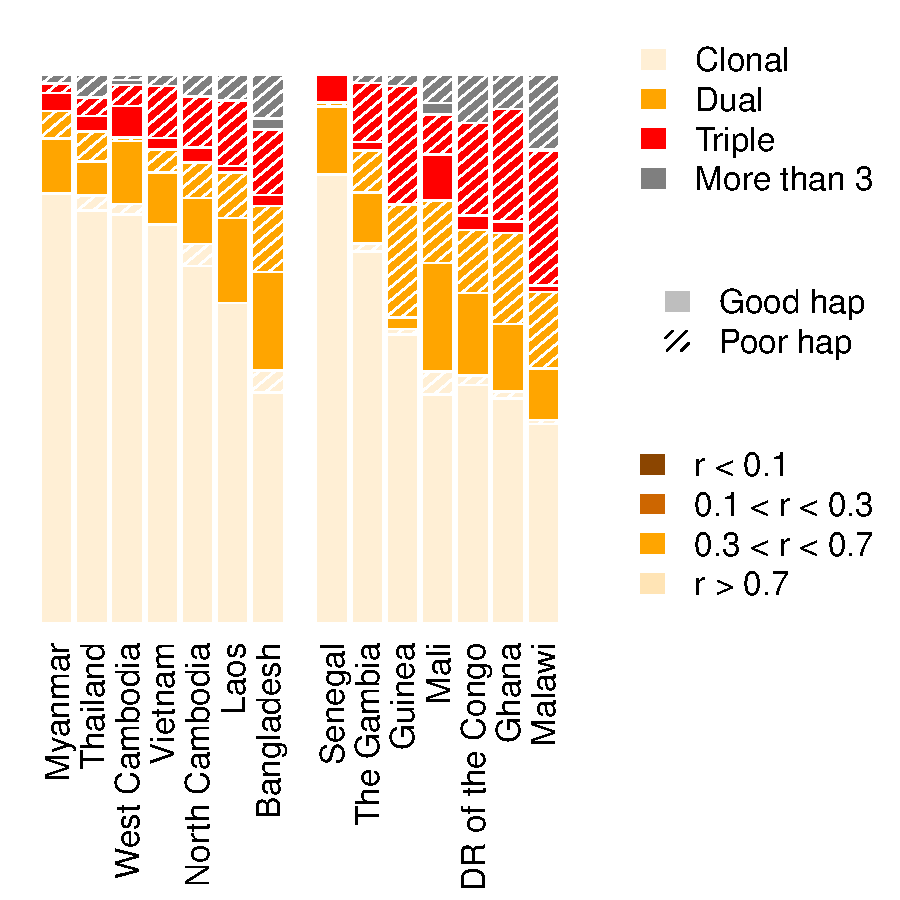
\includegraphics[width=0.36\textwidth]{otherFigures/mixK_after_filtering.pdf}}
  \subfloat[][]{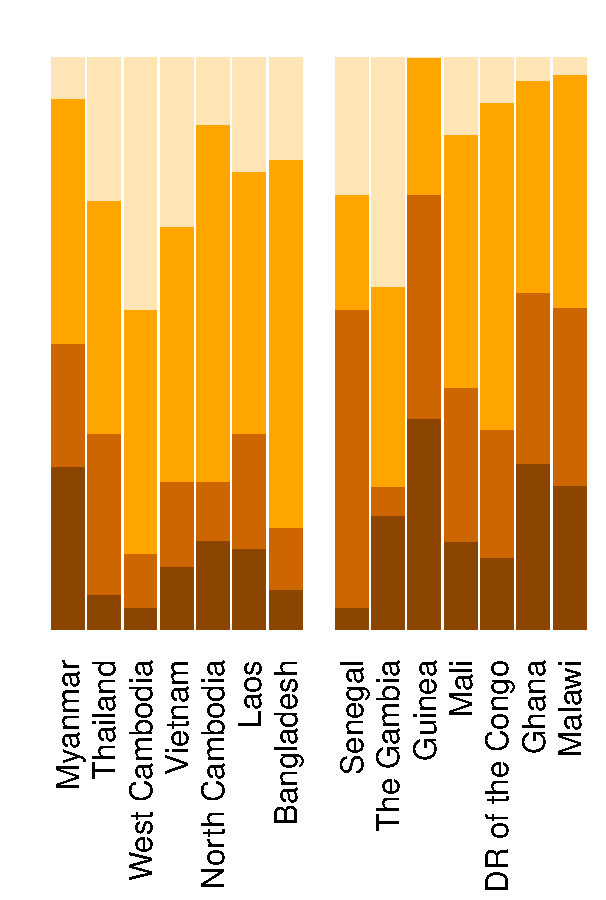
\includegraphics[width=.27\textwidth]{otherFigures/mixIBD_after_filtering.pdf}}
  \subfloat[][]{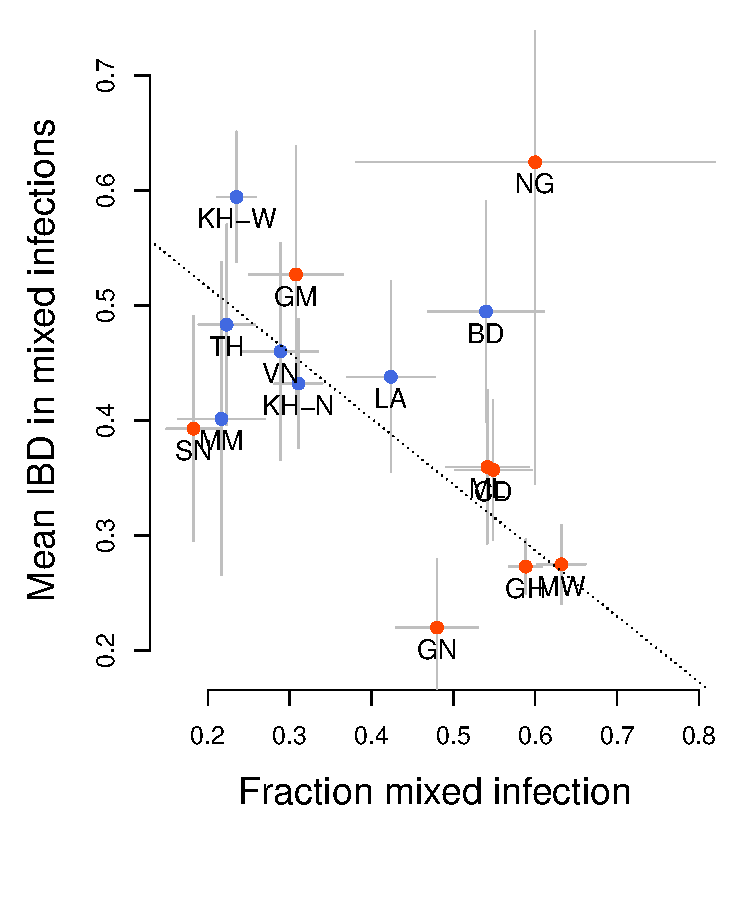
\includegraphics[width=.32\textwidth]{otherFigures/mixInfSum_after_filtering.pdf}}
\end{figure}
\end{document}

